% This section of the handbook was imported from the following work:
% > Cacao ARM-Port Documentation
% > see http://www.cacaojvm.org or http://stud4.tuwien.ac.at/~e0306126/cacao-arm
% > Author: Michael Starzinger <michi@complang.tuwien.ac.at>
% > Projektpraktikum mit Bakkalaureatsarbeit
% > TU Wien, SS 2006

\section{ARM code generator}

This section of the handbook was imported from \emph{``Bakkalaureatsarbeit: Cacao ARM-Port Documentation''}, available at \url{http://stud4.tuwien.ac.at/~e0306126/cacao-arm}

% Version History:
% v0.1: April 13, 2006 (Initial Version)
% v0.2: April 24, 2006 (First Draft)
% v0.3: April 27, 2006 (sent to Andi)
% v0.4: April 29, 2006 (Final Draft)
% v0.5: May 19, 2006 (after Review)

\subsection{About ARM Architecture}
\subsubsection{General}
The ARM processor family (originally the \emph{Acorn RISC Machine}) is a 32-bit RISC architecture with special power saving features. Due to his low power consumption, this processor is most commonly used in embedded systems and mobile electronics. The opcodes have a fixed width of 32 bits.

In contrast to many other RISC machines, the ARM processor has a small amount of registers (16 integer registers). The program counter (PC) is one of these registers and is accessible like any other general purpose register, therefore it can be directly read and written. This allows easy PC-relative addressing, which is commonly used on ARM architectures. A speciality when reading the program counter is the fact that it returns the position of the current instruction plus eight (size of two instructions). 

Another feature is the possibility of \emph{conditional execution} of most instructions. This means machine instructions can be predicated by a special condition which determines whether the instruction is executed or not. This can reduce the amount of branch instructions needed.

\subsubsection{Floating Point Calculation}
The ARM processor is designed to have several co-processors at a time, the instruction set can be arbitrary extended by these co-processors. A standard ARM floating point instruction set has been defined, so that the code may be used across all ARM machines. These standard FP instructions can use up to eight high precision FP registers that can be transfered via registers or memory.

If the actual hardware does not exist, then the instructions are trapped and executed by a floating point emulator. The program itself has no possibility of finding out if a hardware acceleration is present or not.

\subsubsection{Calling Conventions for Linux}
There is an general Application Binary Interface (ABI) available at \cite{ARMabi}, which is a guideline for operating system developers. The ARM port of Linux is almost totally conform to this ABI, so we will simply call them \emph{Linux ABI} from now on.

The conventions themselves will not be discussed here, if you are interested see the appropriate references. However there is a section in this documentation that discusses the special calling conventions inside JIT code.

\subsection{Just-in-Time Code}
This chapter deals with the code produced by the Cacao code generator (from now on referred to as \emph{JIT code}) for ARM processors. The conventions that apply to this code differ from the Linux Calling Conventions in many ways. Special care has to be taken when calling such code from outside. This will be dealt with in a separate chapter. 

The main purpose of these conventions was to be as much conform to the other Cacao ports as possible.

\subsubsection{Code Generation}
Cacao uses intermediate codes for translation, so the code generator translates intermediate codes into ARM machine instructions. It creates instructions by using a set of macros (defined in codegen.h). These macros write one or more instruction into memory and increment the code pointer. The intermediate commands are more or less equivalent to Java byte-code.

\subsubsection{Register Allocation}
Most of the registers are used like expected by the Linux ABI. However, there are some differences. First of all, there are almost no temporary scratch registers on ARM. But most intermediate commands need at least two scratch registers to work properly. One could use argument registers for this purpose, but then arguments needed to be saved. So the decision was to sacrifice three of the callee saved registers and internally (inside JIT code) use them as temporary registers.

\begin{figure}[ht]
\centering
\begin{tabular}{|c|c|c|}
\hline \textbf{ABI Name} & \textbf{Cacao Name} & \textbf{Description} \\
\hline R0 - R3 & A1 - A4 & Argument Registers \\
\hline R4 - R8 & V1 - V5 & Saved Registers \\
\hline R9 & ITMP3 & Temporary Register 3 \\
\hline R10 & ITMP1 & Temporary Register 1 \\
\hline R11 & ITMP2 & Temporary Register 2 \\
\hline R12 (IP) & PV & Procedure Vector \\
\hline R13 (SP) & SP & Stack Pointer \\
\hline R14 (LR) & LR & Link Register (Return Address) \\
\hline R15 (PC) & PC & Program Counter \\
\hline
\end{tabular}
\caption{Register usage inside JIT code}
\label{fig:ARMregs}
\end{figure}

The four argument registers (R0 - R3) are used for argument passing to methods. They can be destroyed inside a method and do not need to be saved. The callee saved registers (R4 - R8) need to be saved and restored by every method.

We have three temporary registers at hand (R9 - R11) which we can use in every intermediate command, there is no need to save these registers at all. Take special care when using ITMP3, this register is �very temporary� and can even be changed by some \emph{load and store instructions} (see codegen.h for further details).

The register R12 (intra-procedure-scratch register, which usually is the only real scratch register) is used as Procedure Vector by our JIT code. It needs to be recomputed after each method or built-in call. This is done by subtracting the relative position of the instruction in our method from the PC. So in a certain way we use PC relative addressing, but do the calculation only once after each method call. Method calls are much less frequent than data-segment accesses, so this makes perfect sense. The remaining three registers (Stack Pointer, Link Register and Program Counter) behave as expected.

\subsubsection{Argument and Result Passing}
The first thing to mention here, is the fact that the ARM port does not differentiate between floating-point arguments and integer arguments. They are both passed exactly the same way and can therefore also be intermixed. Because of the same size, arguments of the type \emph{float} are treated like \emph{integer} and likewise \emph{doubles} as \emph{longs}.

A register is 32 bits long and the stack is also alligned at 32 bits, so \emph{integers} can be passed using one single register or stack space. \emph{Longs} take up 64 bits and are therefore placed in two succeeding registers or two succeeding stack spaces. The endianes of these arguments is thereby defined by the endianes of the machine. 

Result values are not passed unified. Floating-point results are passed using the the floating-point register F0 which can contain a \emph{float} as well as a \emph{double} value. Result values of type \emph{integer} are passed through register R0. For \emph{longs} the two succeeding registers R0 and R1 (according to machine endianes) are used. (Remember that this behavior can change, if \emph{soft-float} is used.)

These calling conventions match with the ones in the Linux ABI, therefore no special care has to be taken when entering or leaving JIT code. Arguments and results can be left at their current places.

\subsubsection{Stack Layout}
The layout of the stack frame that every method needs to have, is totally different from the Linux ABI.

\begin{figure}[ht]
\centering
\begin{tabular}{|c|c|}
\hline \textbf{Description} & \textbf{Size} \\
\hline Saved Link Register & 0 or 1 word \\
\hline Saved Integer Registers & 0 to 5 words \\
\hline Argument for monitorenter() & 0 or 1 word \\
\hline Spilled Registers & 0 to n words \\
\hline
\end{tabular}
\caption{Stack layout inside JIT code}
\label{fig:ARMstack}
\end{figure}

The saved Link Register is a copy of the register R14 (LR) at method entry. Only non-leaf methods (that call other methods or built-ins) need to save this return address, so in special cases it can be omitted.

All callee  saved registers that are destroyed inside our method need to be saved. The register allocator marks these registers. We can store all registers including the Link Register at once with one \emph{store multiple} instruction.

Synchronized methods need to call a \emph{monitorenter} and a \emph{monitorexit}, so the argument to this call needs to be saved as well.

Stack slots that do not fit into ordinary registers are placed onto the stack. This is the last block of our stackframe, it can therefore be used for argument passing as well. 

\subsubsection{Entering and Leaving JIT Code}
The above sections described how the JIT code itself interoperates, but there has to be a point where JIT code is entered the first time and where it is left again. These two intersections need special attention because of the differences in the calling conventions. 

Currently there is only one way to call a JIT method from outside (from C code), namely the use of a special assembler function. First this function saves the temporary registers as mentioned above and prepares the arguments passed to the method. Then it fakes a method invocation as it is usual inside JIT code. This is important because of exception handling (discussed later in this section) and stack tracing. The function also has a data segment like a usual JIT method and an own exception handler to stop stack unwinding before JIT code is left. After the JIT method returns all the stored registers are restored and the calling function doesn't even know what happened.

Methods are compiled right before they are called for the first time, before a method gets compiled it points to s special \emph{compiler stub}. This stub calls another assembler method which saves all argument registers and the return address for the actual method. Then it starts the JIT compiler which actually does the code generation as described in the sections above.

One way to leave JIT code is a patcher call. Cacao needs patchers because some values (like class pointers) are not known during compile time and need to be patched in during runtime. Therefore at some points, jump instructions are placed into the JIT code, which jump to a special \emph{patcher stub}. These stubs prepare a stack-frame with certain information (for the layout of this frame see asmpart.S) and call the \emph{patch wrapper} (a function written in assembler). This wrapper restores the content of every single register, so patchers can be placed nearly everywhere inside the JIT code

Another way to leave JIT code is by throwing an exception, which will invoke the \emph{exception handler} another function written in assembler. This handler tries to unwind the stack by looking at every stack frame and searching the associated method. This is done searching for the instruction block which recomputes the PV (procedure vector) right at the return address after each method invocation. Stored registers and return addresses are restored for each method. If one of the reached methods has an appropriate handler, this handler will get called.

The last way to leave JIT code is by the invocation of a built-in or native method. But since the calling conventions are similar to the Linux ABI, no special care has to be taken here.

\subsection{Pitfalls and other Difficulties}
\subsubsection{Floating Point Issues}
An issue that is commonly overlooked in many implementations for the ARM architecture is a speciality about the way \emph{doubles} are stored in memory on little-endian machines. While the single bytes of this doubles are stored as expected by a little-endian machine, the two 32 bit words of the double are stored big-endian like. This means that the double containing 8 bytes (b0 - b7) in memory at address 100 looks as diagramed in figure \ref{fig:ARMdouble-memory}. Note that this only applies to processors using FPA (floating-point accelerator) or an emulation of such a unit, not to those having a VFP (vector floating-point unit).

\begin{figure}[ht]
\centering
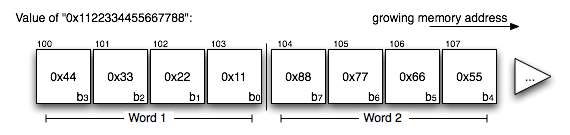
\includegraphics[bb=0 0 570 135, scale=0.6]{arm-double-memory.png} 
\caption{Doubles in memory on little-endian ARMs with FPA}
\label{fig:ARMdouble-memory}
\end{figure}

\subsubsection{Software Floating Point}
Since most ARM machines totally lack a floating-point unit, the corresponding instructions have to be emulated by the operating systems. Linux and most other operating system do this by trapping these instructions and calling a kernel function which does the calculations instead. Even the floating-point registers are available to the programmer.

The huge drawback of this method is the fact that it takes up many CPU cycles to do these kernel calls, which has an extremely negative effect on the overall performance. A possible solution is to not generate floating-point instructions and registers at all. Every computation has to be done by the software itself, this method is called \emph{software floating-point calculation} or simply \emph{soft-float}. When using this mode of code generation, all intermediate codes dealing with floats or doubles are done by certain built-ins which are generated by the compiler (that is used to compile Cacao). This only needs one function call to be made and does not switch to kernel mode at all, therefore it can be considered a huge performance boost on most machines.

Remember that the calling conventions have to change when switching to \emph{soft-float}, since there are no floating-point registers to pass method results. The solution is to use the integer registers R0 and R1 to pass results. In this case \emph{floats} are passed inside R0 and \emph{doubles} are passed using R0 and R1 according to machine endianes.

\subsubsection{Argument Splitting}
There is one speciality of the ARM architecture: \emph{Longs} and \emph{doubles} can be split along the register-stack-barrier when passed as arguments to methods. This means that one word of a \emph{Long} is placed inside a register (register A4 in this case) and the other word is already placed onto the stack (stack space \#0 in this case). This behavior is called \emph{splitted argument} inside the ARM port.

Internally, these splitted arguments are marked as register arguments. The first register is set to A4 as expected, so the register allocator can handle this one normally. The second register is set to a dummy value (SPLIT), which indicates the split and is ignored by the allocator. The allocator does not know where the extra word is located on stack, this is handled by the ARM port itself.

Since such arguments can be reused as stack-slots (like every other register argument), special care had to be taken when loading such stack-slots. An addition check for this constellation had to be inserted.

\subsubsection{Displacement Overflows}
Special care had to be taken when using immediate values on ARM because of the relative small range of such immediates. Constant values (immediates in data processing) are only 8 bits long. So most of the constant values have to be moved onto the data segment (which is right in front of every method and grows towards lower addresses).

There is the possibility of rotating these 8 bits, but this feature is only applicable at few places and therefore merely implemented.

Another aspect where small immediates manifest are offsets to load and store instructions which can only have 12-bit offsets. This occurs quite often, especially because of the heavily growing data segment. Offsets larger than that barrier are called \emph{large displacements} inside Cacao. They are handled by prepending an additional instruction in front of the load or store instruction, which adds or subtracts a rotated immediate from the base register (see codegen.h for further details).

The following figure \ref{fig:ARMdisp-overflow} contains some examples of standard load or store operations as they are very common inside JIT-code and explains how the normal instructions (with small displacement) differ from the extended instructions (with larger displacement)

\begin{figure}[ht]
\centering
\begin{verbatim}
; icmd ACONST (from data-segment) with small displacement:
0x409d07c0:   e51c1038    ldr   r1, [ip, #-56] 

; icmd ACONST (from data-segment) with larger displacement:
0x40da333c:   e24c9a02    sub   r9, ip, #8192   ; 0x2000
0x40da3340:   e5199eb0    ldr   r9, [r9, #-3760] 

; icmd PUTFIELD with normal displacement:
0x409d07d4:   e5863040    str   r3, [r6, #64] 

; icmd PUTFIELD with larger displacement (temp. register R9):
0x409d0fa8:   e2869a09    add   r9, r6, #36864  ; 0x9000
0x409d0fac:   e5893c4c    str   r3, [r9, #3148]  
\end{verbatim}
\caption{Examples of Displacement Overflows}
\label{fig:ARMdisp-overflow}
\end{figure}

\subsubsection{Recalculation of the Procedure Vector}
Another important aspect to be mentioned here is the efficient recalculation of the Procedure Vector (PV) inside JIT-Code. This recalculation has to be done after each method invocation. This includes all Java methods as well as all builtin-calls and other administrative methods like debugging or synchronization methods.

Sine the JIT-Code is assembled as position-independent Code (PIC) this recalculation has to be done in a PC relative fashion. The offset of the current instruction relative to the start of the current method is subtracted from the PC. The value to subtracted in this process can be very large depending on the size of the method, so the shifting ability of of the ARM instruction set can be profitably applied during this calculation.

\begin{figure}[ht]
\centering
\begin{verbatim}
; Recalculation of the PV at relative offset 0x00007c:
0x409d07dc:   e24fcf21    sub   ip, pc, #132    ; 0x84

; Recalculation of the PV at relative offset 0x0151c4:
0x40da336c:   e24fcf73    sub   ip, pc, #460    ; 0x1cc
0x40da3370:   e24ccb54    sub   ip, ip, #86016  ; 0x15000
\end{verbatim}
\caption{Examples of PV recalculation}
\label{fig:ARMrecalculate-pv}
\end{figure}

\subsubsection{Code Patching}
Not all the information needed for program execution is available at compile time. Therefore some parts of the JIT-Code need to be \emph{patched} at runtime. This is accomplished by placing a single branch instruction into the code which overwrites the original instruction at this offset. This branch is replaced by the original instruction by the patcher after the patch has been applied the first time.

Patching can also be accomplished by changing references which are loaded from the data-segment. This is the case after a method has been compiled by the JIT-Compiler for the first to time. To avoid recompilation the refrence to the compiler stub is replaced by the location of the freshly compiled method.

Some of these patchers need to extract information back from already compiled JIT-Code (for example to get the location of the reference to be patched). Therefore patchers need to know the layout of the code very well. Special care has to be taken when changing this layout, all the patchers dealing with it have to be updated as well.

% this is the end of the section 'ARM code generator'
